%---------------------------------------------------------------------------%
%-                                                                         -%
%-                           LaTeX Template                                -%
%-                                                                         -%
%---------------------------------------------------------------------------%
%- Copyright (C) Yuxing Xu <tengyuanchangye222@gmail.com> 
%- This is free software: you can redistribute it and/or modify it
%- under the terms of the GNU General Public License as published by
%- the Free Software Foundation, either version 3 of the License, or
%- (at your option) any later version.
%---------------------------------------------------------------------------%
%->> Document class declaration
%---------------------------------------------------------------------------%
\documentclass[singlesided,fontset=fandol,tikz]{Style/hznuthesis}%
%- Multiple optional arguments:
%- [<singlesided|doublesided|printcopy>]% set one or two sided eprint or print
%- [showmj]% show confidential information
%- [draftversion]% show draft version information
%- [fontset=<fandol|...>]% specify font set to replace automatic detection
%- [scheme=plain]% thesis writing of international students
%- [standard options for ctex book class: draft|paper size|font size|...]%
%---------------------------------------------------------------------------%
%->> Document settings
%---------------------------------------------------------------------------%
\usepackage[super,myhdr,list]{Style/artratex}% document settings
%- usage: \usepackage[option1,option2,...,optionN]{artratex}
%- Multiple optional arguments:
%- [bibtex|biber]% set bibliography processor and package
%- [<numbers|super|authoryear|alpha>]% set citation and reference style
%- <numbers>: textual: Jones [1]; parenthetical: [1]
%- <super>: textual: Jones superscript [1]; parenthetical: superscript [1]
%- <authoryear>: textual: Jones (1995); parenthetical: (Jones, 1995)
%- <alpha>: textual: not available; parenthetical: [Jon95]
%- [geometry]% reconfigure page layout via geometry package
%- [lscape]% provide landscape layout environment
%- [myhdr]% enable header and footer via fancyhdr package
%- [color]% provide color support via xcolor package
%- [background]% enable page background
%- [tikz]% provide complex diagrams via tikz package
%- [table]% provide complex tables via ctable package
%- [list]% provide enhanced list environments for algorithm and coding
%- [math]% enable some extra math packages
\usepackage{Style/artracom}% user defined commands
%---------------------------------------------------------------------------%
%->> Document inclusion
%---------------------------------------------------------------------------%
%\includeonly{Tex/Chap_1,...,Tex/Chap_N}% selected files compilation
%---------------------------------------------------------------------------%
%->> Document content
%---------------------------------------------------------------------------%
\begin{document}
%-
%-> Frontmatter: title page, abstract, content list, symbol list, preface
%-
\frontmatter% initialize the environment
% 导入封面摘要
%---------------------------------------------------------------------------%
%->> Titlepage information
%---------------------------------------------------------------------------%
%-
%-> Chinese titlepage
%-
%\confidential{}% confidential level
\schoollogo{scale=1}{logo}% university logo
\schoolname{scale=0.1}{name}% university name
\graduates{(2019届)}
 %中文标题
  \title{复杂网络理论及其应用}
  \author{许宇星}
  \id{2015210202018}
  \advisor{李安水}
  \advisortitles{讲师}
  \degree{本科}
  \major{信息与计算科学}
  \class{信息151}
  \submitdate{2019年4月30日}
  \defenddate{2019年5月8日}
  \institute{理学院}
  \school{杭州师范大学}
  \score{}
  % 第二页的标题(为英文)
  \englishtitle{Some aspects of complex network theory and its applications}
%-
%-> Create titlepages
%-
\maketitle
\makeenglishtitle



%-
%-> Author's declaration 作者声明
%-
%\makedeclaration
%-
%-> Chinese abstract
%-
\chapter*{摘\quad 要 }

\setcounter{page}{1}% set page number
\pagenumbering{Roman}% set large roman
%楷体
\Abstract{
Facebook、Twitter、微信和微博等社交和信息网络活动已经成为我们日常生活中不可或缺的一部分,在那里,我们可以很容易地接触到朋友的行为,并进而受到朋友的影响。因此,对每个用户进行有效的社会影响预测对于各种应用程序至关重要。传统的社会影响预测方法通常设计各种手工规则来提取特定于用户和网络的特征。然而,它们的有效性在很大程度上取决于领域专家的知识。因此,通常很难将它们推广到不同的领域。

在社交相似性和GHSOM的启发下,本文研究了图特征以及手工特征输入的基于GHSOM的社交影响力算法,学习用户的潜在特征表示,以预测社会影响。将网络结构和特定用户特征在卷积神经网络中补齐。GHSOM将用户的特征作为输出到一个二维的表征网络,以表现其潜在的社会表征。在微博上进行的广泛实验表明,所提出的基于GHSOM的新模型显著优于传统的基于特征工程的方法。}

\keywords{图卷积;GHSOM;社交影响力;社交网络}
%-
%-> English abstract
%-
\chapter*{Abstract}

Social and information networking activities such as on Facebook, Twitter, WeChat, and Weibo have become an indispensable part of our everyday life, where we can easily access friends’ behaviors and are in turn influenced by them. Consequently, an effective social influence prediction for each user is critical for a variety of applications such as online recommendation and advertising.

Conventional social influence prediction approaches typically design various hand-crafted rules to extract user- and network- specific features. However, their effectiveness heavily relies on the knowledge of domain experts. As a result, it is usually difficult to generalize them into different domains. Inspired by social similarity and GHSOM, We design a social influence algorithm based on GHSOM, which has both graph-fixed-point feature and manual feature input. We can learn the representation of users' potential features to predict the social impact. The structure of the network and the user-specific features are complemented in the convolution neural network. GHSOM outputs the user's features into a two-dimensional representation network to represent its potential social representation. Extensive experiments on Weibo show that the proposed GHSOM-based model is significantly superior to the traditional feature-based engineering method.

\englishkeywords{Graph Convolution;Growing Hierarchical Self-Organizing Maps;Social Influence; Social Networks}
%---------------------------------------------------------------------------%
% title page, abstract

{% content list region
\linespread{1.2}% local line space
%\intotoc{\contentsname}% add link to contents table and bookmark

%目录
\tableofcontents% contents catalog
%\intotoc{\listfigurename}% add link to contents table and bookmark

%图形列表
%\listoffigures% figures catalog
%\intotoc{\listtablename}% add link to contents table and bookmark

%表格列表
%\listoftables% tables catalog
}

%->符号列表
%% 符号列表
\chapter*{符号列表}
\chaptermark{符号列表}

\section*{字符}
\nomenclatureitem[\textbf{Unit}]{\textbf{Symbol}}{\textbf{Description}}
\nomenclatureitem[$\Unit{m^{2} \cdot s^{-2} \cdot K^{-1}}$]{$R$}{the gas constant}
\nomenclatureitem[$\Unit{m^{2} \cdot s^{-2} \cdot K^{-1}}$]{$C_v$}{specific heat capacity at constant volume}
\nomenclatureitem[$\Unit{m^{2} \cdot s^{-2} \cdot K^{-1}}$]{$C_p$}{specific heat capacity at constant pressure}
\nomenclatureitem[$\Unit{m^{2} \cdot s^{-2}}$]{$E$}{specific total energy}
\nomenclatureitem[$\Unit{m^{2} \cdot s^{-2}}$]{$e$}{specific internal energy}
\nomenclatureitem[$\Unit{m^{2} \cdot s^{-2}}$]{$h_T$}{specific total enthalpy}
\nomenclatureitem[$\Unit{m^{2} \cdot s^{-2}}$]{$h$}{specific enthalpy}
\nomenclatureitem[$\Unit{kg \cdot m \cdot s^{-3} \cdot K^{-1}}$]{$k$}{thermal conductivity}
\nomenclatureitem[$\Unit{kg \cdot m^{-1} \cdot s^{-2}}$]{$S_{ij}$}{deviatoric stress tensor}
\nomenclatureitem[$\Unit{kg \cdot m^{-1} \cdot s^{-2}}$]{$\tau_{ij}$}{viscous stress tensor}
\nomenclatureitem[$\Unit{1}$]{$\delta_{ij}$}{Kronecker tensor}
\nomenclatureitem[$\Unit{1}$]{$I_{ij}$}{identity tensor}

\section*{算子}
\nomenclatureitem{\textbf{Symbol}}{\textbf{Description}}
\nomenclatureitem{$\Delta$}{difference}
\nomenclatureitem{$\nabla$}{gradient operator}
\nomenclatureitem{$\delta^{\pm}$}{upwind-biased interpolation scheme}

\section*{缩写}
\nomenclatureitem{CFD}{Computational Fluid Dynamics}
\nomenclatureitem{CFL}{Courant-Friedrichs-Lewy}
\nomenclatureitem{EOS}{Equation of State}
\nomenclatureitem{JWL}{Jones-Wilkins-Lee}
\nomenclatureitem{WENO}{Weighted Essentially Non-oscillatory}
\nomenclatureitem{ZND}{Zel'dovich-von Neumann-Doering}

% list of symbols, preface content
%-
%-> Mainmatter
%-
% 论文主体
\mainmatter% initialize the environment
%---------------------------------------------------------------------------%
%->> Main content
%---------------------------------------------------------------------------%

\chapter{绪论}

\label{chap:introduction}
社会影响无处不在,不仅存在于我们的日常生活中,也存在于虚拟网络空间中。“社会 影响”一词通常指一个人的情绪、观点或行为受到他人影响的现象。随着在线和移动社交平台的全球普及,人们已经看到了社会影响在各个领域的影响,如总统选举\cite{2012political}、广告\cite{v011a004}等等。到目前为止,毫无疑问,社会影响已经成为推动我们社会决策的一种普遍而复杂的力量,明确需要方法来描述、理解和量化社会影响的基本机制和动态。


\begin{figure}[!htbp]
    \centering
    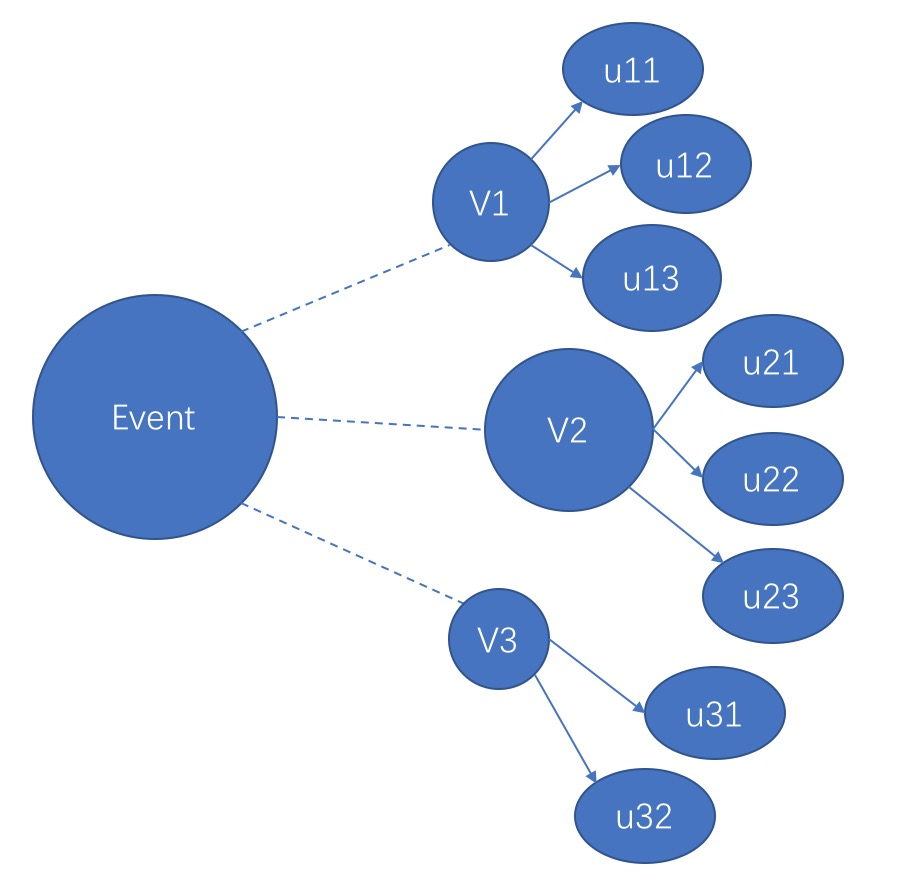
\includegraphics[width=0.50\textwidth]{Event}
    \caption{热点事件传播示意图}
    \label{fig:Event}
\end{figure}

\section{研究现状}\label{sec:status}

事实上,许多文献都对社会影响预测做了大量的工作。例如,Matsubara等人\cite{Rise2012fall}通过精心设计从经典的“易感染”模型扩展而来的微分方程,研究了社会影响的动力学。最近,Li等人\cite{DBLP:journals/corr/LiMGM16}出了一种结合递归神经网络(RNN)和表示学习来推断级联大小的端到端预测方法。所有这些方法的主要目的是预测社会影响的全球或聚集模式,如在一个时间框架内的级联规模。然而,在许多在线应用中,如广告和推荐,有效地预测每个人的社会影响是至关重要的,即用户层面的社会影响预测。像Twitter这样的西方在线社交网络已经得到了很好的研究,但中国人气颇高的微博网络新浪微博的特点却一直很少被研究过。文献\cite{2012arXiv1202.0327Y}发现,转发在新浪微博上更加普遍,并为创造趋势做出了很大贡献。

国内文献\cite{2019TSRank}\cite{2016PSO}\cite{2018UserInfluenc}\cite{2015similarity}尝试对于微博社交影响力进行多个角度的研究。其中文献\cite{2016PSO}提出将粒子群算法应用于热点话题的发现,得出结果表明用户的转发操作对话题的影响力有比较大的影响的结论。文献\cite{2019TSRank}考虑用户话题信息传播能力以及用户与背景话题间关联性,提出了TSRank算法,但是上述论文都没有考虑使用者在整个社群网络结构中的各种重要程度。



本文主要研究用户层面的社会影响预测。我们的目的是通过某一热点话题在转发过程中不同用户的行动状态,用户的近邻的动作状态和该话题被转发的的结构信息,给出该热点话题的影响力。例如,在图\ref{fig:Event}中,当热点事件发生之后,常常是社区中的意见领袖刷线发布原创内容,经过普通用户层层传递,持续活跃直至周期结束。

\begin{figure}[!htbp]
    \centering
    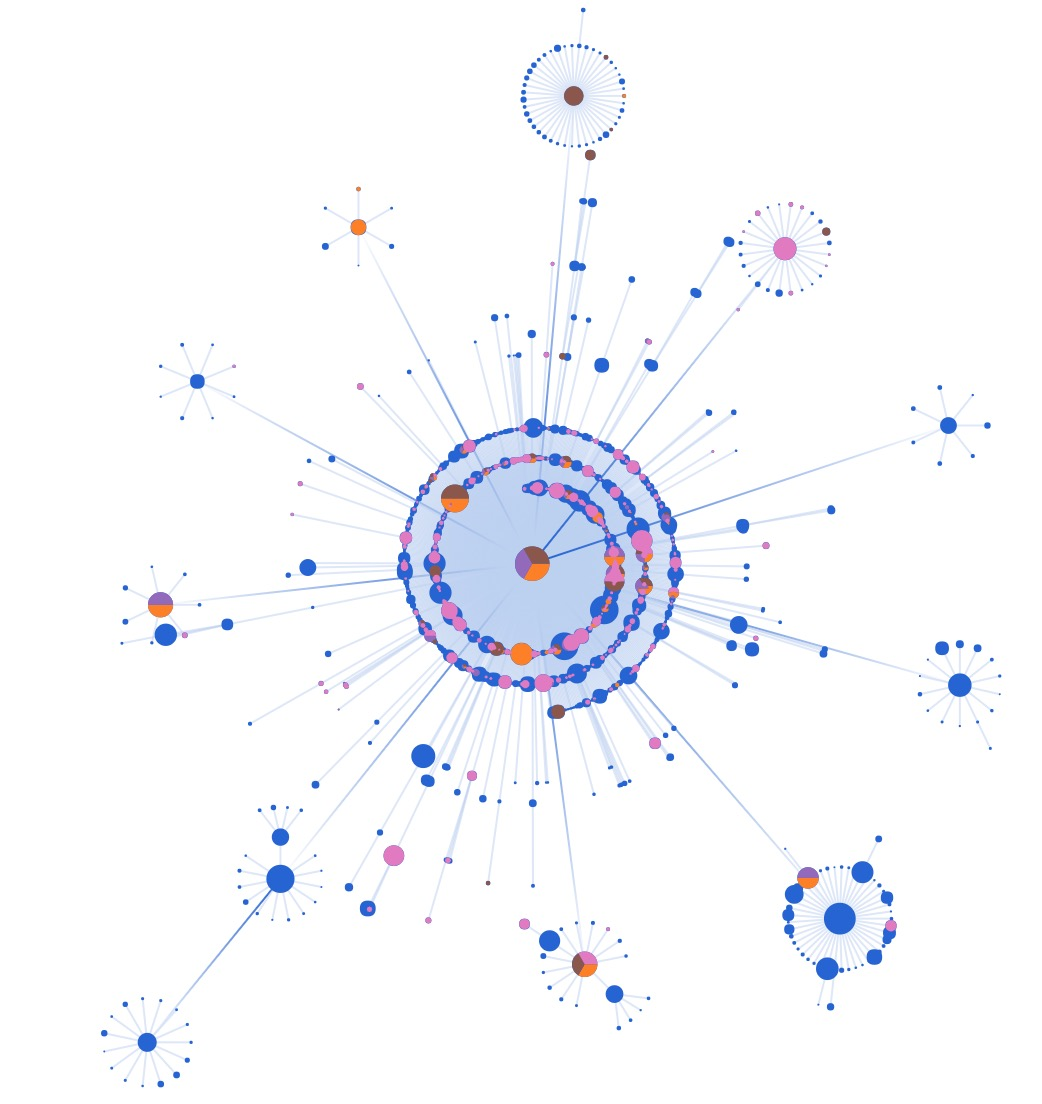
\includegraphics[ width=0.50\textwidth]{Circular}
    \caption{社交用户转发关系图(不同的颜色表示不同关键词)}
    \label{fig:Circular}
\end{figure}

受到社交相似性在微博转发中的预测成功的启发\cite{2015similarity},我改进了基于GHSOM\cite{2018UserInfluenc}算法,发现社会影响中隐藏的和预测的信号。通过将网络嵌入\cite{Qiu:2018:NEM:3159652.3159706}、图卷积\cite{kipf2017semi}和SOM神经网络构建到一个方案中。在获得如图\ref{fig:Circular}所示的转发网络后,我们利用图卷积技术来补齐关键特征。然后经过GHSOM神经网络将高维特征中隐藏的信息映射到二维网络上,结合网络特征和自定义的手工特征计算社会影响力。经过广泛的实验,结果表明,模型可以方法能准确及有效评估微博用户的影响力。

\newtheorem{theorem}{定义}[subsection]
\section{问题特征}\label{sec:question}

\subsection{顶点特征}
\begin{theorem}[度中心性]
连结度中心性为该节点与其邻居节点的所有连结数的总合。
\end{theorem}
如式(\ref{con:degreeCentrality})所示。
\begin{equation}
C_D(n_i)=degree_{in}(n_i)+degree_{out}(n_i)
\label{con:degreeCentrality}
\end{equation}
式(\ref{con:degreeCentrality})中,$degree_{in}(n_i)$ 代表其 他使用者连到$n_i$使用者的连结数,$degree_{out}(n_i)$为使用者$n_i$连到其他使用者的连结数。



\begin{theorem}[邻近度中心性]
邻近度中心性则是以该节点与其余所有在同一网络中的节点的距离总和来做计算。
\end{theorem}
\begin{equation}
C_c(n_i)=\frac{1}{\sum_{k\neq1} distance(n_i,n_j)}
\label{con:closenessCentrality}
\end{equation}
如式(\ref{con:closenessCentrality})所示。式(\ref{con:closenessCentrality})中,$distance(n_i,n_j)$为$n_i$到$n_j$节点的距离。





\begin{theorem}[中介度中心性]
中介度中心性则是用来计算除了该节点外的所有节点中,任两节点之间的路径中,通过该节点的路径数除以此两节点所有路径数比值的总合。
\end{theorem}
当节点在网络 中扮演着链接两个原先互不相连的节点之角色时,该节点中介度中心性的值则会较高,
\begin{equation}
C_B(n_i)=\sum_{j,k\neq i}\frac{|path_{via n_i}(n_i,n_k)|}{|path_{total}(n_j,n_k)|}
\label{con:betweennessCentrality}
\end{equation}
如式(\ref{con:betweennessCentrality})所示。式(\ref{con:betweennessCentrality})中,$path_{via n_i}(n_i,n_k)$为节点$n_j$通过节点$n_i$而连结到节点$n_k$的最短路径数,$path_{total}(n_j,n_k)$则为节点$n_j$连 结到节点$n_k$的所有最短路径数。





\subsection{手工特征}

Repost influence 则是用户本月所 发布的信息被转发次数的平均,该项指针能反映出使 用者所发布之言论的价值。
式(\ref{con:repostInf})中,
$N_m$为使用者每月所发布之信息量,而$\sum N_R$则为每月 每则信息被转发次数之总和。
\begin{equation}
I_r=1-\sqrt{\frac{N_m}{N_m+\sum N_R}}
\label{con:repostInf}
\end{equation}

Repost depth 转发深度,用章节\ref{sec:analyse}中的被转发的层数的最大值来评估。


Mention influence 为用户每月所发布之信息被 回复及评论的次数,该项指标反映出使用者能吸引多 少追随者来参与对话的能力,也就是言论话题性。
式(\ref{con:mentionInf})中,$N_M$为使用者每月所发布之信息
量,$\sum N_M$则为每月每则信息被讨论次数之总和。
\begin{equation}
I_m=1-\sqrt{\frac{N_m}{N_m+\sum N_M}}
\label{con:mentionInf}
\end{equation}


Geographical influence 地理影响分布,参考\href{https://open.weibo.com/wiki/%E7%9C%81%E4%BB%BD%E5%9F%8E%E5%B8%82%E7%BC%96%E7%A0%81%E8%A1%A8}{新浪微博的省份城市编码},比如,宁夏的省份编号是64,其下的主要城市分别为1银川、2石嘴山、3吴忠、4固原,青海的省份编号是63,其下主要城市有8个。我们发现地理上相邻的省份及城市,其编号也非常接近,我们建立影响广度特征公式(\ref{con:geoInf})。其中$P$表示省份,$C$表示城市,$I_{i,j}$表示在省份P下的城市C被影响的个数。
\begin{equation}
I_g=\frac{1}{P}\sum_{i\in P}\sum_{j\in C}\frac{I_{i,j}}{I_{i,total}}
\label{con:geoInf}
\end{equation}


检验预测结果的方法。
Spearman’s rank correlation coefficients是用来 分析两种排名算法之间相关性的量测方法。
如式(\ref{con:spearman})所示。该分析方法是根据等级数据研究两个变量间相关 性的方法,相关性越高其分析结果越接近+1,相关性 越低其分析结果越接近-1。

\begin{equation}
\rho=1-\sqrt{\frac{6\sum (x_i-y_i)}{N(N^2-1)}}
\label{con:spearman}
\end{equation}

%\newtheorem{theorem}{定义}[section]
\chapter{问题特征}
\label{chap:formulation}
在这一部分中,我们引入必要的定义,主要分为图结构特征和手工特征,然后制定预测社会影响的问题。
\section{顶点特征}
\begin{theorem}[度中心性]
连结度中心性为该节点与其邻居节点的所有连结数的总合。
\end{theorem}
如式\ref{con:degreeCentrality}所示。式\ref{con:degreeCentrality}中,$degree_{in}(n_i)$ 代表其 他使用者连到$n_i$使用者的连结数,$degree_{out}(n_i)$为使用者$n_i$连到其他使用者的连结数。
\begin{equation}
C_D(n_i)=degree_{in}(n_i)+degree_{out}(n_i)
\label{con:degreeCentrality}
\end{equation}




\begin{theorem}[邻近度中心性]
邻近度中心性则是以该节点与其余所有在同一网络中的节点的距离总和来做计算
\end{theorem}
如式\ref{con:closenessCentrality}所示。式\ref{con:closenessCentrality}中,$distance(n_i,n_j)$为$n_i$到$n_j$节点的距离。
\begin{equation}
C_c(n_i)=\frac{1}{\sum_{k\neq1} distance(n_i,n_j)}
\label{con:closenessCentrality}
\end{equation}





\begin{theorem}[中介度中心性]
中介度中心性则是用来计算除了该节点外的所有节点中,任两节点之间的路径中,通过该节点的路径数除以此两节点所有路径数比值的总合。
\end{theorem}
当节点在网络 中扮演着链接两个原先互不相连的节点之角色时,该 节点中介度中心性的值则会较高,如下式\ref{con:betweennessCentrality}所示。式\ref{con:betweennessCentrality}中,$path_{via n_i}(n_i,n_k)$为节点$n_j$通过节点$n_i$而连结到节点$n_k$的最短路径数,$path_{total}(n_j,n_k)$则为节点$n_j$连 结到节点$n_k$的所有最短路径数。
\begin{equation}
C_B(n_i)=\sum_{j,k\neq i}\frac{|path_{via n_i}(n_i,n_k)|}{|path_{total}(n_j,n_k)|}
\label{con:betweennessCentrality}
\end{equation}






\section{手工特征}
Repost influence 则是用户本月所 发布的信息被转发次数的平均,该项指针能反映出使 用者所发布之言论的价值。
式\ref{con:repostInf}中,
$N_m$为使用者每月所发布之信息量,而$\sum N_R$则为每月 每则信息被转发次数之总和。
\begin{equation}
I_r=1-\sqrt{\frac{N_m}{N_m+\sum N_R}}
\label{con:repostInf}
\end{equation}

Repost depth 转发深度,用章节\ref{sec:analyse}中的被转发的层数的最大值来评估。


Mention influence 为用户每月所发布之信息被 回复及评论的次数,该项指标反映出使用者能吸引多 少追随者来参与对话的能力,也就是言论话题性。
式\ref{con:mentionInf}中,$N_M$为使用者每月所发布之信息
量,$\sum N_M$则为每月每则信息被讨论次数之总和。
\begin{equation}
I_m=1-\sqrt{\frac{N_m}{N_m+\sum N_M}}
\label{con:mentionInf}
\end{equation}


Geographical influence 地理影响分布,参考\href{https://open.weibo.com/wiki/%E7%9C%81%E4%BB%BD%E5%9F%8E%E5%B8%82%E7%BC%96%E7%A0%81%E8%A1%A8}{新浪微博的省份城市编码},比如,宁夏的省份编号是64,其下的主要城市分别为1银川、2石嘴山、3吴忠、4固原,青海的省份编号是63,其下主要城市有8个。我们发现地理上相邻的省份及城市,其编号也非常接近,我们建立影响广度特征公式\ref{con:geoInf}。其中$P$表示省份,$C$表示城市,$I_{i,j}$表示在省份P下的城市C被影响的个数。
\begin{equation}
I_g=\frac{1}{P}\sum_{i\in P}\sum_{j\in C}\frac{I_{i,j}}{I_{i,total}}
\label{con:geoInf}
\end{equation}


检验预测结果的方法。
Spearman’s rank correlation coefficients是用来 分析两种排名算法之间相关性的量测方法。
如式\ref{con:spearman}所示。该分析方法是根据等级数据研究两个变量间相关 性的方法,相关性越高其分析结果越接近+1,相关性 越低其分析结果越接近-1。

\begin{equation}
\rho=1-\sqrt{\frac{6\sum (x_i-y_i)}{N(N^2-1)}}
\label{con:spearman}
\end{equation}


\chapter{主要模型}
\label{chap:model}
这一部分将会依次介绍GCN\cite{kipf2017semi}、GHSOM\cite{2018UserInfluenc}、特征量化模型,为下一节实验做准备。我将经过GCN处理的数据作为GHSOM的输入,将高未特征映射到二维空间,结合特征量化模型输出影响力数值。将影响力排名与微博话题榜做比较,使得斯皮尔曼的等级相关系数最大化。

\section{GCN模型}\label{sec:model1}

图卷积神经网络是一种用于图形结构数据的半监督学习算法。通过叠加多个GCN层建立GCN模型。每个GCN层的输入是一个顶点特征矩阵,$H\in \mathbb{R}^{n\times F}$,其中n是顶点数,F是特征数,每行 H,用$h_i^T$表示,与一个顶点相关联。一般来说,GCN层的本质是一个非线性变换,输出如下$H'\in \mathbb{R}^{n\times F}$:
\begin{equation}
H'=GCN(H)=g(A(G)HW^T+b)
\end{equation}
其中$W\in \mathbb{R}^{F'\times F}$,$𝑏 \in \mathbb{R}^{F'}$是模型参数,g 为非线性激活函数,A(G)为获取图 G 结构信息 的 n×n 矩阵,GCN 将A(G)实例化为与归一化图 Laplaican密切相关的静态矩阵:
\begin{equation}
A_{GCN(H)} = D^{-1/2}AD^{-1/2}
\end{equation}
其中 A 是 G 的邻接矩阵,$D=diag(A1)$是度矩阵。

引入一个简单而又灵活的图信息传播模型$f(X,A)$,我们可以返回到半监督节点分类问题。我们可以放宽通常在基于图的半监督学习中所作的某些假设,方法是对数据X和底层图结构的邻接矩阵A对我们的模型$f(X,A)$进行条件调整。在邻接矩阵包含不存在于数据X中的信息的场景中,例如引用网络中的文档之间的引用链接或知识图中的关系时,通常期望这种设置特别强大。总体模型,一个用于半监督学习的多层GCN。



我们首先在预处理步骤中计算$\widehat{A}=\widetilde{D}^{(-1/2)}\widetilde{A}\widetilde{D}^{(-1/2)}$。然后,我们的传播模型采用了简单的形式:
\begin{equation}
Z=f(X,A)=softmax(\widehat{A}ReLU(\widehat{A}XW^{(0)})W^{(1)})
\end{equation}
这里,$W^{(0)}\in \mathbb{R}^{C\times H}$是一个具有H特征映射的隐藏层的输入到输出的权矩阵。$W^{(1)}\in \mathbb{R}^{C\times H}$是一个隐输出权矩阵。Softmax激活函数,定义为$softmax(X_i)=\frac{1}{Z}exp(X_i),Z=\sum_{i}exp(X_i)$,逐行应用。对于半监督的多类分类,对所有标号样本的交叉熵误差进行了评估:
\begin{equation}
\mathcal{L}=-\sum_{l\in y_L}\sum_{f=1}^{F}Y_{lf}lnZ_{lf},
\end{equation}
其中$Y_L$是一组具有标签的节点索引。利用梯度下降训练神经网络权值$W^{(0)}$和$W^{(1)}$。


\section{GHSOM模型}\label{sec:model2}

GHSOM网络是建立在SOM的基础上的一种延伸模型。
简单地说,自组织映射是一种实现竞争学习的人工神经网络,可以认为是一种无监督学习形式。在地图上,神经元沿着$x_{dim}$和$y_{dim}$维数的矩形网格排列。对于每个训练实例$\vec{x}_k,k=1,2,3,...,M$,M是训练实例的数目。

1、竞争步骤,在矩形网格上找到特定训练实例的最佳匹配神经元,
\begin{equation}
c=argmin_{i}(|| \vec{x}_i-\vec{x}_k||),
\end{equation}

其中$i,k=1,2,3,...,N$是MAP神经元上的一个指数,$N=x_{dim}×y_{dim}$是网格上的神经元数,$\vec{m}_i$是i索引的神经元。最后,c是映射上最佳匹配神经元的指标。

2、更新步骤,训练实例$\vec{x}_k$影响最佳匹配神经元$\vec{m}_c$及其邻域。更新步骤可以由地图上神经元的以下更新规则表示,
\begin{equation}
\vec{m}_i\gets \vec{m}_i-\eta \vec{\delta}_ih(c,i)
\end{equation}

即$i=1,2,...,N$,这里$\vec{\delta}=\vec{m}_i-\vec{x}_k$,$\eta$是学习速率,$h(c,i)$是一个损失函数,
\begin{equation}
h(c,i)=\left\{
\begin{aligned}
1 &  & if~i \in \Gamma(x), \\
0 &  & otherwise ,
\end{aligned}
\right.
\end{equation}

其中$\Gamma(c)$是最佳匹配神经元$\vec{m}_c$与$c\in \Gamma(c)$的邻域。通常情况下,邻居是时间的函数,它的大小在训练期间衰减。最初,神经元$\vec{m}_c$的邻域包括地图上的所有其他神经元,
\begin{equation}
\Gamma(c)|_{t=0}={1,2,...,N},
\end{equation}

随着训练的进行,$\vec{m}_c$的邻域缩小到仅限于神经元本身,
\begin{equation}
\Gamma(c)|_{t\gg0}={c},
\end{equation}

在这里,像以前一样,$N=x_{dim}×y_{dim}$是映射上的神经元数。这意味着每个最佳匹配神经元的更新规则最初都有一个很大的影响范围,逐渐缩小到影响域只包含最佳匹配神经元本身的程度。

对每个训练实例重复上述两个训练步骤,直到给定的映射收敛为止。

在SOM中,输出层的类神经网络单元是以一维或二维矩阵的方式排列,并根 据输入向量彼此竞争,获胜的神经元称之为优胜神经元,其可获得调整权重向量的机会,经过数个迭代的权重调整后,输出层的神经元便会呈现出代表输入向量特征的拓扑结构( topology) 。

增长阶层式自组织映像图(以下简称GHSOM)增长阶层式自组织映像图模型是SOM的一种延伸模型,整体呈现多层次的阶层式结构,每层又由数个能自我调适的 SOM 所构成...


GHSOM克服了固定大小数据的映射方式的限制; 因此,即使是在没有先验知识的情况下,依然可以提供最令人满意的结果的网络架构。由于所有数据都映射在不同的二维空间中,因此层次关系清晰。




\chapter{实验设置}
\label{chap:experiment}

我们利用大规模的真实数据集进行了实验,以定量评估所提出的算法框架。

\section{数据集}\label{sec:dataset}
我们的实验在微博的社交网络上进行。微博是中国最受欢迎的社交平台之一。
数据集来自网络爬虫\cite{Ren2014WeiboEvents},数据包含了微博id、微博作者id、微博发布时间以及评论数转发数等相当多的特征。完整的数据格式和各字段意义见附录。

使用tkipf-GCN框架\cite{kipf2017semi}还支持多个图实例(可能不同大小)的分批分类,每个实例都有一个邻接矩阵。最好是将各自的特征矩阵连接起来,并建立一个(稀疏)块对角矩阵,其中每个块对应于一个图实例的邻接矩阵。

这是模型的运行结果图,随着迭代次数的增加,过了500个epoch左右后,用训练数据测量到的识别精度几乎都为 100\%。但是,对于测试数据,离100\%的识别精度还有较大的差距。如此大的识别精度差距,是只拟合了训练数据的结果。出现了的过拟合现象(如图\ref{fig:epoch}),再经过正则化修正之后,选取迭代次数为200性能的GCN网络。
\begin{figure}[!htbp]
    \centering
    \begin{subfigure}[b]{0.35\textwidth}
      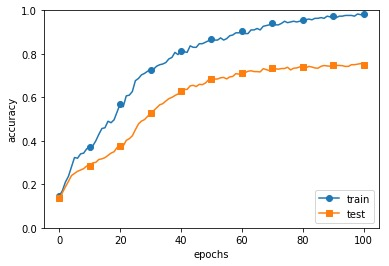
\includegraphics[width=\textwidth]{epoch100}
      \caption{}
      \label{fig:epoch100}
    \end{subfigure}%
    ~%add desired spacing
    \begin{subfigure}[b]{0.35\textwidth}
      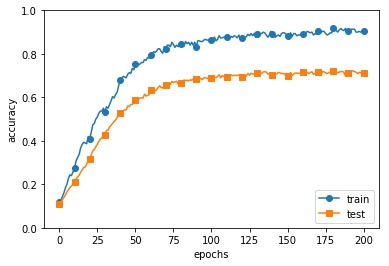
\includegraphics[width=\textwidth]{epoch200}
      \caption{}
      \label{fig:epoch200}
    \end{subfigure}%
    \begin{subfigure}[b]{0.35\textwidth}
      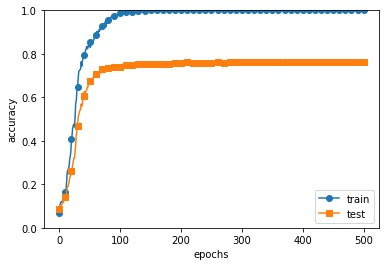
\includegraphics[width=\textwidth]{epoch500}
      \caption{}
      \label{fig:epoch500}
    \end{subfigure}%

    \caption{预测准确率,(a) 迭代次数为100次的GCN预测准确率,(b) 迭代次数为200次,(c) 迭代次数为500次。}
    \label{fig:epoch}
\end{figure}
该网络预测的准确率稳定在75\%左右,满足我们的实验要求。一份无特征缺失的数据保障了实验的进行。


这里,我们将处理过后的数据进行时间和空间尺度上的分析,下面是分析结果的可视化。
\begin{figure}[!htbp]
    \centering
    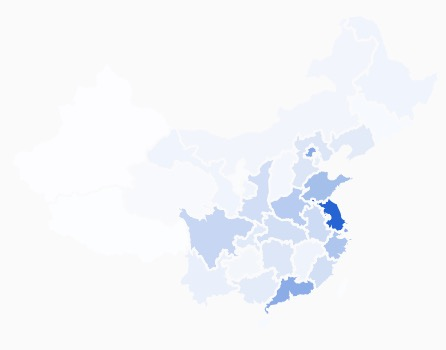
\includegraphics[width=0.50\textwidth]{Position}
    \caption{微博用户的地理分布}
    \label{fig:Position}
\end{figure}
图\ref{fig:Position}是微博用户的位置的可视化。从图\ref{fig:Position}中可以看出,该事件转发评论的微博用户主要集中在沿海地区,江苏尤为集中,内陆以四川、河南为代表,总体来说经济发达地区对此事件关注度普遍较高。因此,我们认为地理距离也是衡量社交相似性的一个重要特征。具体可以查看数据中省份城市编码,对照新浪微博的开发文档中的省份城市编码表。


时间尺度分析:
\begin{figure}[!htbp]
    \centering
    \begin{subfigure}[b]{0.5\textwidth}
      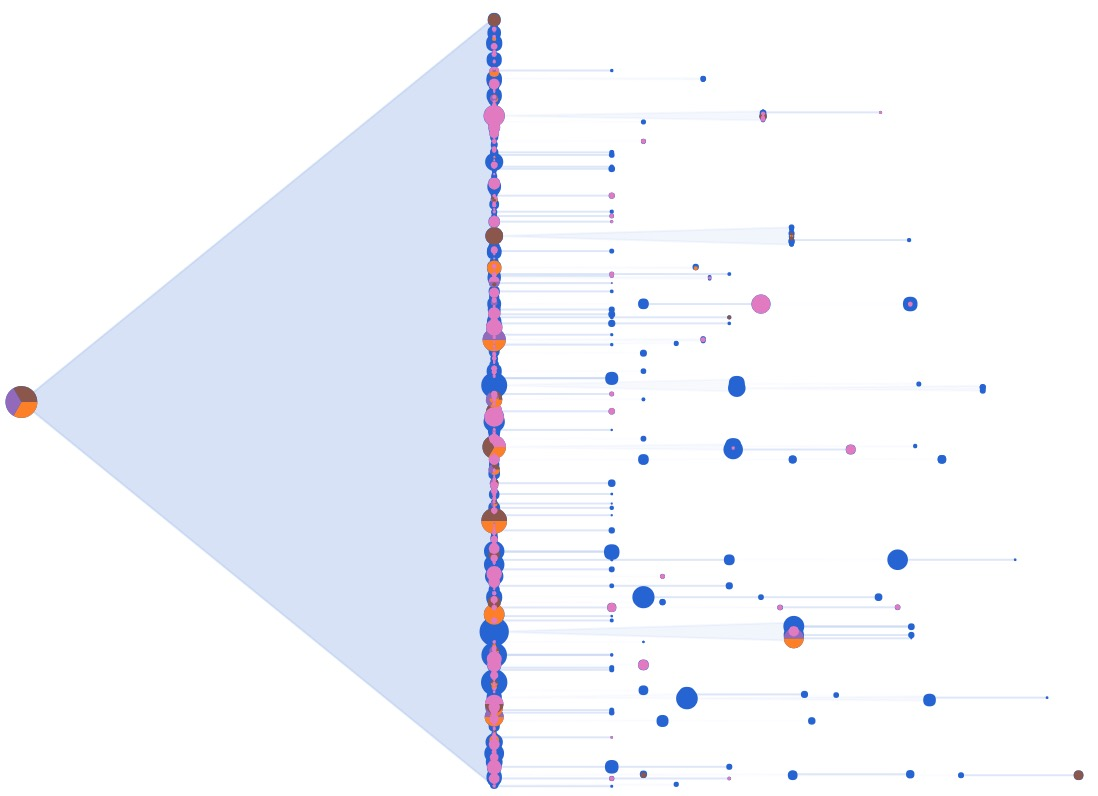
\includegraphics[width=\textwidth]{Tree}
      \caption{}
      \label{fig:Tree}
    \end{subfigure}%
    ~%add desired spacing
    \begin{subfigure}[b]{0.5\textwidth}
      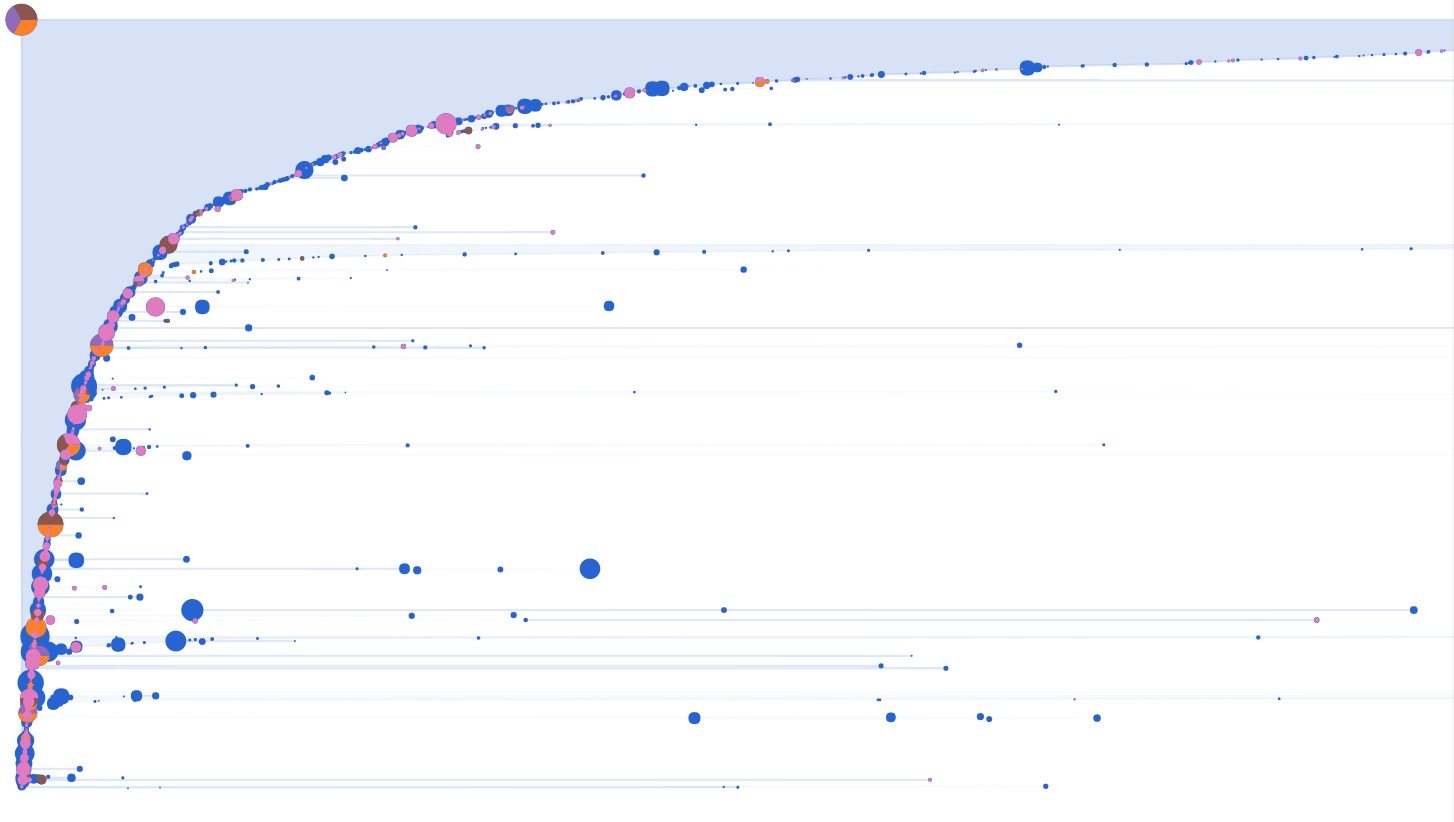
\includegraphics[width=\textwidth]{Sail}
      \caption{}
      \label{fig:Sail}
    \end{subfigure}%

    \caption{(a) 树形图,(b) 船帆图。}
    \label{fig:Time}
\end{figure}
如图\ref{fig:Time}所示。图\ref{fig:Tree}反映了各个转发层数随着时间的分布。通过观察我们可以发现,大多数意见领袖都处于第一层转发者,事件最多经过了7层转发。可见转发层数也是衡量一个事件影响力的重要特征。图\ref{fig:Sail}反映了各个转发节点随着时间的分布。



关键节点分析:如图\ref{fig:Repost}。图\ref{fig:Repost}中可以清楚地观察到事件的核心社交圈以及各个子社交圈的意见领袖及其分布。由此我们通过分析意见领袖的领域分布及其在各自领域的影响力来得出各个子社交圈的影响力。这些意见领袖在各自社交圈的影响力也成为了评估事件影响力的一个重要特征。
\begin{figure}[!htbp]
    \centering
    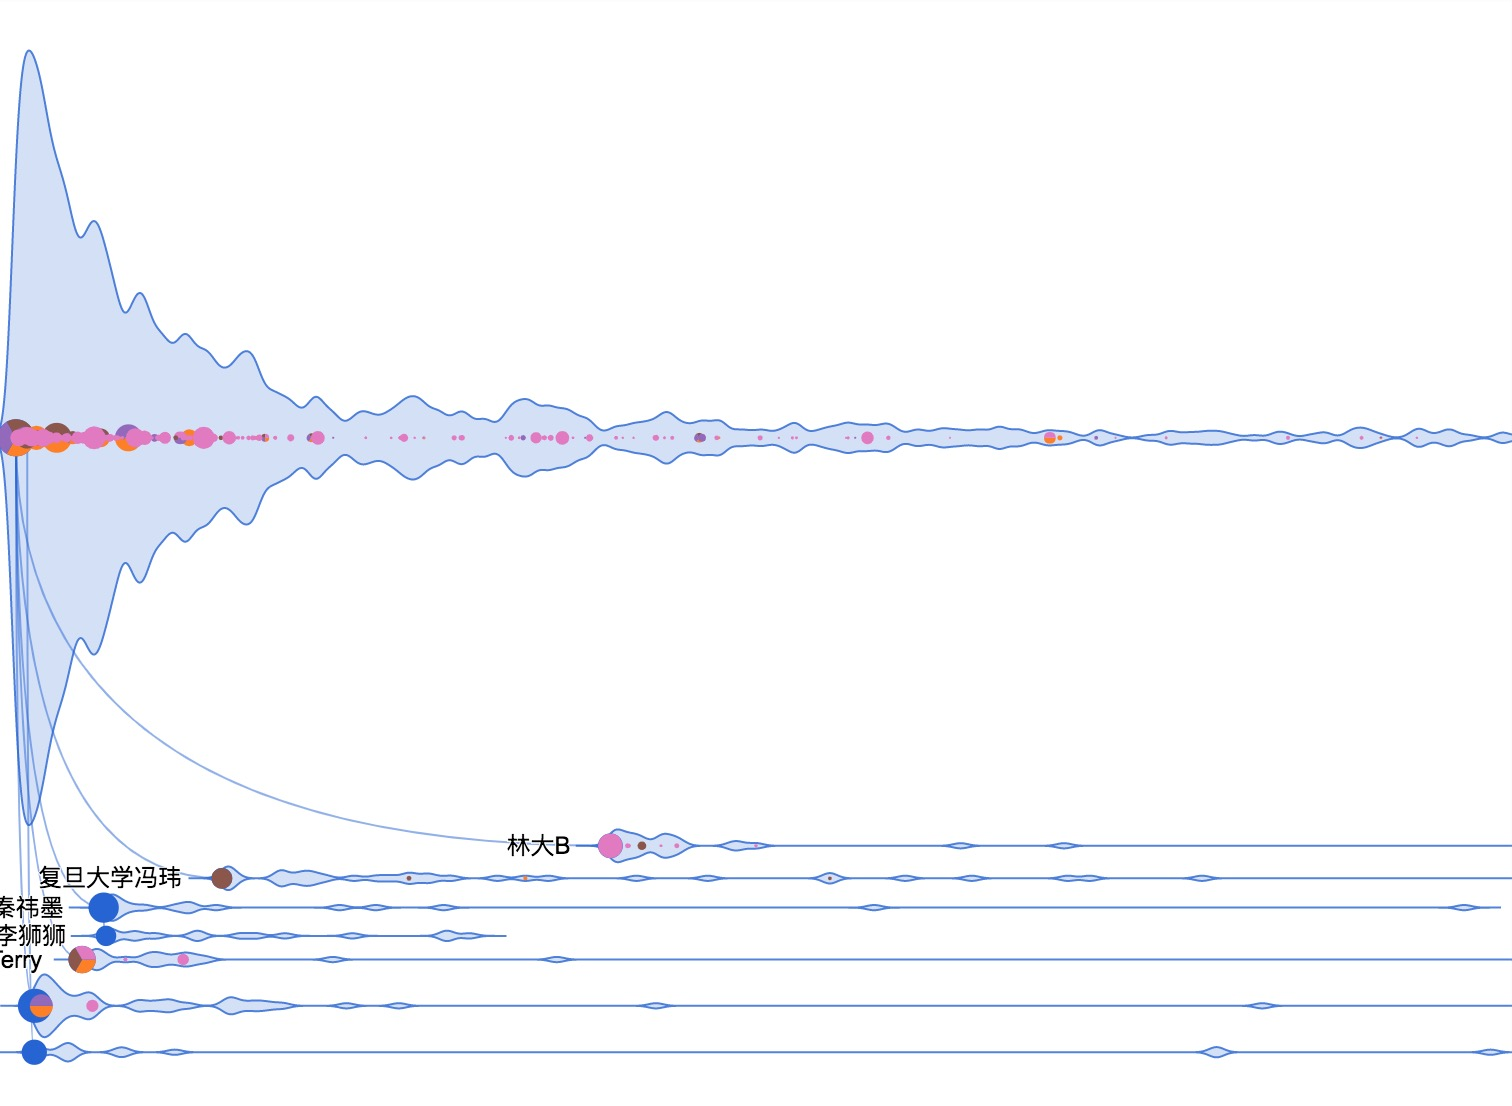
\includegraphics[width=0.5\textwidth]{Curves}
    \caption{话题热度随时间变化示意图}
    \label{fig:Curves}
\end{figure}
热度分析:




\section{评估指标}
为了定量评估本文的算法,我们使用以下性能指标:

预测性能~我们评估预测性能根据曲线下面积(AUC)、精度(Prec)、召回(Rec)和 F1 测量(F1)。

参数灵敏度~我们分析了我们的模型和测试不同的超参数选择如何影响预测性能。 

案例研究~我们使用具体案例来进一步证明和解释我们提出的算法的有效性。


\section{算法比较}

我们将GHSOM与几个算法进行比较。

逻辑回归(LR)使用逻辑回归(LR)来训练。该模型考虑了三类特征:(1)用户的顶点特征;(2)预训练网络嵌入;(3)手工制作的网络特征。

支持向量机(SVM)使用了支持向量模型。以线性核为分类模型的机器(SVM)。该模型使用与逻辑回归(LR)相同的特征。








\chapter{实验结果}
\label{chap:result}

我们比较了上一节中所提到的方法的预测性能,并列出了表4 (AUC)、精度(Prec)、召回(Rec)和 F1 测量(F1)。并结合两个实际的案例来探索其应用价值。
请见表




\section{参数调整}\label{sec:anly}

GHSOM中的超参数主要有初始映像图大小、广度参数和深度参数这三个。
通过实际的数据,观察不同的初始映像图大小会在多大程度上影响神经网络的学习。这里基于不同初始映像图大小进行实验。结果如图\ref{fig:initialization}所示。

\begin{figure}[!htbp]
    \centering
    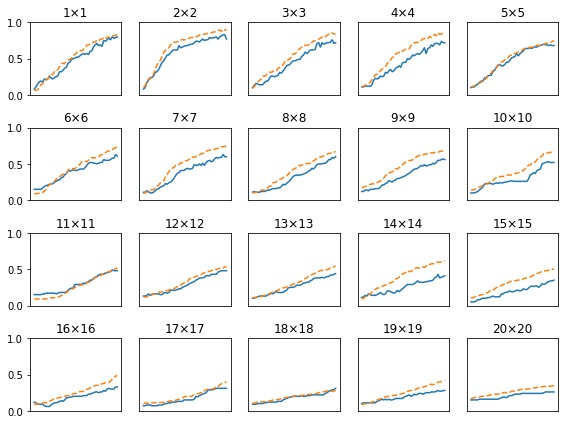
\includegraphics[width=0.8\textwidth]{sominit}
    \caption{实线是验证数据的识别精度,虚线是训练数据的识别精度}
    \label{fig:initialization}
\end{figure}


从图\ref{fig:initialization}中,按识别精度从高到低的顺序排列了验证数据的学习的变化。从图中可知,直到“4×4”左右,学习进行得都很顺利。因此,我们来 观察一下“4×4”之前的超参数的值(学习率),结果如下表\ref{tab:init}所示。从这个结果可以看出,学习率在 0.001 到 0.01时,学习可以顺利进行。


\begin{table}[!htbp]
    \caption{实验结果}
    \label{tab:init}
    \centering
    \footnotesize% fontsize
    \setlength{\tabcolsep}{4pt}% column separation
    \begin{tabular}{l*{5}{c}r}
        size       & val acc  & lr  \\
        \hline
        1×1        & 0.83     & 0.0092  \\
        2×2        & 0.78     & 0.00956 \\
        3×3        & 0.77     & 0.00571 \\
        4×4        & 0.74     & 0.00626 \\
    \end{tabular}
\end{table}

\section{算法应用}
本章节将从舆情监控和广告投放两方面的案例进行分析。

\subsection{舆情监控}
在这一部分中,将本文算法得出的结果与微博名下的大数据监控平台微热点的相关分析结果做比较。微热点将微博话题简单的分成了政治、经济、法治、教育、商业、民生、医疗、交通、文娱和体育十大板块。

我们根据系统架构所提出的方法,提取2019年3月21日下午14时48分左右江苏盐城爆炸事件相关微博,该事件至论文完成时已经累积2.6亿次阅读,属于突发事件。部分微博机构、用户的影响力占比如下表所示。





\subsection{广告投放}

某著名微博营销网站采用的用户投放报价方式,是基于传统的转发、评论、点赞,如图所示..



\chapter{相关工作}
\label{chap:relative}

我们的研究与大量关于社会影响分析和图形表征学习的文献密切相关...

\chapter{结论}
\label{chap:conclusion}

在这项工作中,研究了社会影响的时空分布、领域分布、地域分布等问题。我们从机器学习的角度来阐述这个问题,并结合最新开发的网络嵌入、图形卷积技术,提出了一个基于图形的分析框架。我在微博上测试了该算法的框架。广泛的实验分析表明,GHSOM在预测话题社会影响方面明显优于。本文探讨了GHSOM网络表征学习在社会影响分析中的潜力,并尝试解释微博话题的动态社会影响...

\chapter{使用简介}
\label{chap:guide}

\section{数学公式、图表、参考文献等功能}

\subsection{数学公式}

比如Navier-Stokes方程:
\begin{equation} \label{eq:ns}
    \begin{cases}
        \frac{\partial \rho}{\partial t} + \nabla\cdot(\rho\Vector{V}) = 0 \\
        \frac{\partial (\rho\Vector{V})}{\partial t} + \nabla\cdot(\rho\Vector{V}\Vector{V}) = \nabla\cdot\Tensor{\sigma}\\
        \frac{\partial (\rho E)}{\partial t} + \nabla\cdot(\rho E\Vector{V}) = \nabla\cdot(k\nabla T) + \nabla\cdot(\Tensor{\sigma}\cdot\Vector{V})
    \end{cases}
\end{equation}

数学公式常用命令请见 \href{https://en.wikibooks.org/wiki/LaTeX/Mathematics}{WiKibook Mathematics}。artracom.sty中对一些常用数据类型如矢量矩阵等进行了封装,这样的好处是如有一天需要修改矢量的显示形式,只需单独修改artracom.sty中的矢量定义即可实现全文档的修改。

\subsection{表格}

请见表~\ref{tab:sample}。制表的更多范例,请见 \href{https://en.wikibooks.org/wiki/LaTeX/Tables}{WiKibook Tables}。
\begin{table}[!htbp]
    \bicaption{这是一个样表。}{This is a sample table.}
    \label{tab:sample}
    \centering
    \footnotesize% fontsize
    \setlength{\tabcolsep}{4pt}% column separation
    \renewcommand{\arraystretch}{1.2}%row space 
    \begin{tabular}{lcccccccc}
        \hline
        Row number & \multicolumn{8}{c}{This is a multicolumn} \\
        %\cline{2-9}% partial hline from column i to column j
        \hline
        Row 1 & $1$ & $2$ & $4$ & $5$ & $6$ & $7$ & $8$\\
        Row 2 & $1$ & $2$ & $4$ & $5$ & $6$ & $7$ & $8$\\
        Row 3 & $1$ & $2$ & $4$ & $5$ & $6$ & $7$ & $8$\\
        Row 4 & $1$ & $2$ & $4$ & $5$ & $6$ & $7$ & $8$\\
        \hline
    \end{tabular}
\end{table}

\subsection{图片插入}

插图的参考代码在\verb|Tex/Commands.tex|亦进行了汇集。

\subsection{算法}

如见算法~\ref{alg:euclid},详细使用方法请参见文档 \href{https://ctan.org/pkg/algorithmicx?lang=en}{algorithmicx}。

\begin{algorithm}[!htbp]
    \small
    \caption{Euclid's algorithm}\label{alg:euclid}
    \begin{algorithmic}[1]
        \Procedure{Euclid}{$a,b$}\Comment{The g.c.d. of a and b}
        \State $r\gets a\bmod b$
        \While{$r\not=0$}\Comment{We have the answer if r is 0}
        \State $a\gets b$
        \State $b\gets r$
        \State $r\gets a\bmod b$
        \EndWhile\label{euclidendwhile}
        \State \textbf{return} $b$\Comment{The gcd is b}
        \EndProcedure
    \end{algorithmic}
\end{algorithm}

\subsection{参考文献引用}

参考文献引用过程以实例进行介绍,假设需要引用名为"Document Preparation System"的文献,步骤如下:

1)使用Google Scholar搜索Document Preparation System,在目标条目下点击Cite,展开后选择Import into BibTeX打开此文章的BibTeX索引信息,将它们copy添加到ref.bib文件中(此文件位于Biblio文件夹下)。

2)索引第一行 \verb|@article{lamport1986document,|中 \verb|lamport1986document| 即为此文献的label (\textbf{中文文献也必须使用英文label},一般遵照:姓氏拼音+年份+标题第一字拼音的格式),想要在论文中索引此文献,有两种索引类型:

文本类型:\verb|\citet{lamport1986document}|。正如此处所示 \citet{MLin2016complexnet}; 

括号类型:\verb|\citep{lamport1986document}|。正如此处所示 \citep{MLin2016complexnet}。

\textbf{多文献索引用英文逗号隔开}:

\verb|\citep{lamport1986document,chen2005zhulu}|。正如此处所示 \citep{MLin2016complexnet,Ren2014WeiboEvents}

如此,即完成了文献的索引,请查看下本文档的参考文献一章,看看是不是就是这么简单呢?是的,就是这么简单!

不同文献样式和引用样式可在Thesis.tex中对artratex.sty调用实现,如:
\begin{itemize}
    \footnotesize
    \item \verb+\usepackage[numbers]{artratex}+ $\%$ 文本: Jones [1]; 括号: [1]
    \item \verb+\usepackage[super]{artratex}+ $\%$ 文本: Jones 上标[1]; 括号: 上标[1]
    \item \verb+\usepackage[authoryear]{artratex}+ $\%$ 文本: Jones (1995); 括号: (Jones, 1995)
    \item \verb+\usepackage[alpha]{artratex}+ $\%$ 文本: 不可用; 括号: [Jon95]
\end{itemize}

若在上标(super)模式下,希望在特定位置将上标改为嵌入式标,可使用

文本类型:\verb|\citetns{lamport1986document,chen2005zhulu}|。

正如此处所示\citetns{lamport1986document,chen2005zhulu}

括号类型:\verb|\citepns{lamport1986document,chen2005zhulu}|。

正如此处所示\citepns{lamport1986document,chen2005zhulu}

参考文献索引更为详细的信息,请见 \href{https://en.wikibooks.org/wiki/LaTeX/Bibliography_Management}{WiKibook Bibliography}。

\nocite{*}

\section{常见使用问题}\label{sec:qa}

\begin{enumerate}
    \item 模板每次发布前,都已在Windows,Linux,MacOS系统上测试通过。下载模板后,若编译出现错误,则请遵从 \href{https://github.com/mohuangrui/ucasthesis}{位于主页底部的用户指南}。

    \item 模板文档的编码为UTF-8编码。所有文件都必须采用UTF-8编码,否则编译后生成的文档将出现乱码文本。若出现文本编辑器无法打开文档或打开文档乱码的问题,请检查您使用的编辑器对UTF-8编码的支持。如果使用WinEdt作为文本编辑器(不推荐使用),应在其Options -> Preferences -> wrapping选项卡下将两种Wrapping Modes中的内容:
        
        TeX;HTML;ANSI;ASCII|DTX...
        
        修改为:TeX;\textbf{UTF-8|ACP;}HTML;ANSI;ASCII|DTX...
        
        同时,取消Options -> Preferences -> Unicode中的Enable ANSI Format。

    \item 推荐选择xelatex或lualatex编译引擎编译中文文档。编译脚本的默认设定为xelatex编译引擎。你也可以选择不使用脚本编译,如直接使用 \TeX{}文本编辑器编译。注:\TeX{}文本编辑器编译的默认设定为pdflatex编译引擎,若选择xelatex或lualatex编译引擎,请进入下拉菜单选择。为正确生成引用链接,需要进行全编译。
    \item Texmaker使用简介
        \begin{enumerate}
            \footnotesize
            \item 使用 Texmaker “打开” Thesis.tex。
            \item 菜单 “选项 (Options)” -> “设置当前文档为主文档 (Define as Master Document)”
            \item 菜单 “自定义 (User)” -> “自定义命令 (User Commands)” -> “编辑自定义命令 (Edit User Commands)” -> 左侧选择 “command 1”,右侧 “菜单项 (Menu Item)” 填入 Auto Build -> 点击下方“向导 (Wizard)” -> “添加 (Add)”: xelatex + bibtex + xelatex + xelatex + pdf viewer -> 点击“完成 (OK)”
            \item 使用 Auto Build 编译带有未生成引用链接的源文件,可以仅使用 xelatex 编译带有已经正确生成引用链接的源文件。
            \item 编译完成,“查看(View)” PDF,在pdf中 “ctrl+click” 可链接到相对应的源文件。
        \end{enumerate}
    
    \item 模版的设计可能地考虑了适应性。致谢等所有条目都是通过最为通用的

        \verb+\chapter{item name}+  and \verb+\section*{item name}+

        来显式实现的 (请观察Backmatter.tex),从而可以随意添加,放置,和修改,如同一般章节。对于图表目录名称则可在ucasthesis.cfg中进行修改。

    \item 设置文档样式: 在artratex.sty中搜索关键字定位相应命令,然后修改
        \begin{enumerate}
            \item 正文行距:启用和设置 \verb|\linespread{1.5}|,默认1.5倍行距。
            \item 参考文献行距:修改 \verb|\setlength{\bibsep}{0.0ex}|
            \item 目录显示subsection:修改 \verb|\setcounter{tocdepth}{2}|
            \item 文档超链接的颜色及其显示:修改 \verb|\hypersetup|
            \item 页眉页脚设定:frontmatterstyle,mainmatterstyle,和backmatterstyle分别定义前言,主要内容,和附录的页眉页脚样式。通过阅读这一部分的代码,可以轻松地理解和修改以获得自定义的样式。命令的详细解释请参见 \href{https://www.ctan.org/pkg/fancyhdr?lang=en}{fancyhdr} 的用户文档。同时可参见 \href{https://ctan.org/pkg/ctex?lang=en}{ctex} 宏包用户文档。

            \item 设置图2.3为图2-3: 设置
                {
                    \footnotesize
\begin{verbatim}
\renewcommand{\theequation}{\arabic{chapter}-\arabic{equation}}
\renewcommand{\thefigure}{\arabic{chapter}-\arabic{figure}}
\renewcommand{\thetable}{\arabic{chapter}-\arabic{table}}
\end{verbatim}
                }
        \end{enumerate}

    \item 字体控制。文档内字体切换方法:
        \begin{itemize}
            \item 宋体:飞扬跋扈~或 \textrm{飞扬跋扈}
            \item 粗宋体:{\bfseries 飞扬跋扈} 或 \textbf{飞扬跋扈}
            \item 黑体:{\sffamily 飞扬跋扈} 或 \textsf{飞扬跋扈}
            \item 粗黑体:{\bfseries\sffamily 飞扬跋扈} 或 \textsf{\bfseries 飞扬跋扈}
            \item 仿宋:{\ttfamily 飞扬跋扈} 或 \texttt{飞扬跋扈}
            \item 楷体:{\itshape 飞扬跋扈} 或 \textit{飞扬跋扈}
        \end{itemize}
        
        由于缺乏一个统一的被各个操作系统所默认携带的完备的中文字体库,\href{https://ctan.org/pkg/ctex?lang=en}{ctex} 针对不同的操作系统而调用各系统上所对应的一类中文字体库。由于很多操作系统的字库往往缺乏原生态的加粗宋体字重,有时会发生加粗宋体被黑体所替换的情形,这对封面的字体造成影响。若需要解决这个问题,可采用调用自定义的一个完备字体库的方案。若需设置字体库,请选择xelatex或lualatex编译引擎,并设置需要的字体库。
        
        如\textbf{用Times New Roman作为英文和数字字体},在artratex.sty的

        \verb|\RequirePackage{fontspec}|

        行下添加如下英文字体调用命令:

        \verb|\setmainfont{Times New Roman}| (设置英文正文字体)

        \verb|\setsansfont{Times New Roman}| (设置英文标题字体)

        Windows和Mac OS自带此字体,Linux需手动安装或使用FreeSerif字体作为替代。部分\LaTeX{}版本,若setmainfont与setsansfont调用同一字体名称,会导致字体冲突,进而导致非加粗黑体失效,影响目录及节标题的显示。解决此问题的办法为1)不设置setsansfont 或 2)调用一个名字不同的Times类字体,如setsansfont\{Times\},其中Times字体为Mac OS所带有。长图表标题的英文标题的悬挂缩进是针对Times类正文字体校准的,非Times类正文字体将存在轻微位置偏差。
                 
        如果需要调用一个\textbf{自定义的中文字体库},方法为:

        \begin{itemize}
            \item 调用 \href{https://ctan.org/pkg/ctex?lang=en}{ctex} 预定义好的备用字库: 在Thesis.tex中设置

                {
                    \small\verb|\documentclass[doublesided,fontset=fandol]{Style/ucasthesis}%|
                }

                便可调用 \href{https://ctan.org/tex-archive/fonts/fandol?lang=en}{fandol} 这一字体库。\LaTeX{}编译系统一般已携带或是能自动下载安装 \href{https://ctan.org/tex-archive/fonts/fandol?lang=en}{fandol} 字库。若不能,则请手动下载并安装链接所提供的所有字体即可。本模板使用说明文档就是采用调用 \href{https://ctan.org/tex-archive/fonts/fandol?lang=en}{fandol} 中文字库。

            \item 手动调用系统带有的中文字库: 首先需要查看系统所带有的中文字库及其名称,也可选择安装可获得的中文字库。假设系统已安装或带有名为SC的中文字库(此字库为MacOS所配备,具备原生态的加粗宋体),则可在artratex.sty的

                \verb|\RequirePackage{fontspec}|

                行下添加如下中文字体调用命令:
                {
                    \scriptsize
\begin{verbatim}
\setCJKmainfont[BoldFont=Songti SC Bold,ItalicFont=Kaiti SC]{Songti SC Light}%
\setCJKsansfont{Heiti SC}%
\end{verbatim}
                }
        \end{itemize}

        字库调用的全面解释可参见 \href{https://ctan.org/pkg/fontspec}{fontspec} (英文字体调用)和 \href{https://ctan.org/pkg/xecjk?lang=en}{xeCJK} (中文字体调用)。因为模版的设定考虑兼顾不同操作系统(Windows, Linux, Mac OS),为了模版的健壮性,上述字体设置和调用方案并未作为原始设定。

    \item 封面下划线上的文本不居中下划线,这是因为那些下划线前面还有字头,导致文本只能在页面居中和在下划线上居中二选一。当前封面采取页面居中。如需要调整文本在下划线上的位置,可用 \verb|\hspace{+/- n.0em}| 命令来插入或删除 n 个空格,进行手动调整,比如

        \verb|\advisor{\hspace{+3.0em} xxx~研究员~xxx单位}|
                
                这个解决方案是很不优雅,但问题本质还是样式的设计问题。有时下划线看上去粗细不一致,这是显示的问题,打印正常。

    \item 对于电子档的论文,在Thesis.tex的documentclass中,可使用singlesided来减少空白页。而对于打印版,可考虑printcopy选项使奇偶页的排版在打印装订后更美观。

    \item 部分所也许对格式有不同设定,因\LaTeX{}将内容与格式分离,格式的调整可独立于内容进行,并只需修改模板样式文件完成,并无风险。
\end{enumerate}



%---------------------------------------------------------------------------%
% main content
%-
%-> Appendix
%-
%\cleardoublepage%
%\appendix% initialize the environment
%\renewcommand{\algorithmicrequire}{\textbf{Input:}}  % Use Input in the format of Algorithm  
\renewcommand{\algorithmicensure}{\textbf{Output:}} % Use Output in the format of Algorithm  

\chapter[附  录]{附录}
\chaptermark{附录}
\section*{数据说明}
\nomenclatureitem[\textbf{说明}]{}{\textbf{字段名称}}
\nomenclatureitem[微博的 ID]{1}{$id$}
\nomenclatureitem[微博的 MID]{2}{$mid$}
\nomenclatureitem[微博作者的 UID]{3}{$uid$}
\nomenclatureitem[该条微博直接转发微博的MID]{4}{$parent$}
\nomenclatureitem[微博的类型]{5}{$type$}
\nomenclatureitem[微博发布时间,Unix Timestamp]{6}{$t$}
\nomenclatureitem[微博的评论数]{6}{$comments_{count}$}
\nomenclatureitem[微博的转发数]{7}{$reposts_{count}$}
\nomenclatureitem[微博作者创建时间]{8}{$user_{created}$}
\nomenclatureitem[微博作者的粉丝数]{9}{$followers_{count}$}
\nomenclatureitem[微博作者的微博数]{10}{$statuses_{count}$}
\nomenclatureitem[微博作者的关注数]{11}{$friends_{count}$}
\nomenclatureitem[微博作者的用户名]{12}{$username$}
\nomenclatureitem[作者的用户描述]{13}{$user_{description}$}
\nomenclatureitem[微博作者的城市编号]{14}{$city$}
\nomenclatureitem[微博作者的省份编号]{15}{$province$}
\nomenclatureitem[作者的性别m为男f为女n为未知]{16}{$gender$}
\nomenclatureitem[微博作者是否已加V]{17}{$verified$}
\nomenclatureitem[微博作者加V原因]{18}{$verified_{reason}$}
\nomenclatureitem[微博加V类型]{19}{$verified_{type}$}
\nomenclatureitem[微博文本]{20}{$original_{text}$}
\nomenclatureitem[作者本人文本]{21}{$text$}
\nomenclatureitem[分词结果]{22}{$words$}
\nomenclatureitem[情感分析]{23}{$emotion$}

%\section*{缩写}
%\nomenclatureitem{BFS}{Breadth First Search}
%\nomenclatureitem{DFS}{Depth First Search}
%\nomenclatureitem{GHSOM}{Growing Hierarchical Self-Organizing Maps}
%\nomenclatureitem{PSO}{Particle Swarm Optimization}

\section*{伪代码}

\begin{algorithm}[!htbp]
    \small
    \caption{The node2vec algorithm}\label{alg:node2vec}
    \begin{algorithmic}[1]
        \Function{LearnFeatures}{Graph $G=(V,E,W)$,Dimensions $d$,Walks per node r,Walk length $l$,Context size $k$,Return $p$,In-out $q$}
        \State $\pi=PreprocessModifiedWeights(G,p,q)$
        \State $G'=(V,E,\pi)$
        \State Initialize $walks$ to Empty

        \For{$iter=1~to~r$ }
        	\ForAll{ nodes $u \in V$}
        	\State $walk=node2vecWlak(G',u,l)$ 
        	\State $walk~to~walks$
        	\EndFor 
        \EndFor
        \State $f=StochasticGradientDescent(k,d,walks$)
        \State\Return $f$ 
        \EndFunction
    \end{algorithmic}
 
    \begin{algorithmic}[1]
        \Function{node2vecWalk}{Graph $G'=(V,E,\pi)$,Start node $u$,Length $l$}
        \State Initialize $walks$ to [u]
        \For{$walk\_iter=1~to~l$}
        \State $curr=walk[-1]$
        \State $V_{curr} =GetNeighbors(surr,G')$
        \State $s=AliasSample(V_{curr},\pi)$
        \State Append $s~to~walk$
        \EndFor
        \State \Return $walk$
        \EndFunction
    \end{algorithmic}

\end{algorithm}



% appendix content
%-
%-> Backmatter: bibliography, glossary, index
%-
% 初始化环境
\backmatter% initialize the environment
%附录
\renewcommand{\algorithmicrequire}{\textbf{Input:}}  % Use Input in the format of Algorithm  
\renewcommand{\algorithmicensure}{\textbf{Output:}} % Use Output in the format of Algorithm  

\chapter[附  录]{附录}
\chaptermark{附录}
\section*{数据说明}
\nomenclatureitem[\textbf{说明}]{}{\textbf{字段名称}}
\nomenclatureitem[微博的 ID]{1}{$id$}
\nomenclatureitem[微博的 MID]{2}{$mid$}
\nomenclatureitem[微博作者的 UID]{3}{$uid$}
\nomenclatureitem[该条微博直接转发微博的MID]{4}{$parent$}
\nomenclatureitem[微博的类型]{5}{$type$}
\nomenclatureitem[微博发布时间,Unix Timestamp]{6}{$t$}
\nomenclatureitem[微博的评论数]{6}{$comments_{count}$}
\nomenclatureitem[微博的转发数]{7}{$reposts_{count}$}
\nomenclatureitem[微博作者创建时间]{8}{$user_{created}$}
\nomenclatureitem[微博作者的粉丝数]{9}{$followers_{count}$}
\nomenclatureitem[微博作者的微博数]{10}{$statuses_{count}$}
\nomenclatureitem[微博作者的关注数]{11}{$friends_{count}$}
\nomenclatureitem[微博作者的用户名]{12}{$username$}
\nomenclatureitem[作者的用户描述]{13}{$user_{description}$}
\nomenclatureitem[微博作者的城市编号]{14}{$city$}
\nomenclatureitem[微博作者的省份编号]{15}{$province$}
\nomenclatureitem[作者的性别m为男f为女n为未知]{16}{$gender$}
\nomenclatureitem[微博作者是否已加V]{17}{$verified$}
\nomenclatureitem[微博作者加V原因]{18}{$verified_{reason}$}
\nomenclatureitem[微博加V类型]{19}{$verified_{type}$}
\nomenclatureitem[微博文本]{20}{$original_{text}$}
\nomenclatureitem[作者本人文本]{21}{$text$}
\nomenclatureitem[分词结果]{22}{$words$}
\nomenclatureitem[情感分析]{23}{$emotion$}

%\section*{缩写}
%\nomenclatureitem{BFS}{Breadth First Search}
%\nomenclatureitem{DFS}{Depth First Search}
%\nomenclatureitem{GHSOM}{Growing Hierarchical Self-Organizing Maps}
%\nomenclatureitem{PSO}{Particle Swarm Optimization}

\section*{伪代码}

\begin{algorithm}[!htbp]
    \small
    \caption{The node2vec algorithm}\label{alg:node2vec}
    \begin{algorithmic}[1]
        \Function{LearnFeatures}{Graph $G=(V,E,W)$,Dimensions $d$,Walks per node r,Walk length $l$,Context size $k$,Return $p$,In-out $q$}
        \State $\pi=PreprocessModifiedWeights(G,p,q)$
        \State $G'=(V,E,\pi)$
        \State Initialize $walks$ to Empty

        \For{$iter=1~to~r$ }
        	\ForAll{ nodes $u \in V$}
        	\State $walk=node2vecWlak(G',u,l)$ 
        	\State $walk~to~walks$
        	\EndFor 
        \EndFor
        \State $f=StochasticGradientDescent(k,d,walks$)
        \State\Return $f$ 
        \EndFunction
    \end{algorithmic}
 
    \begin{algorithmic}[1]
        \Function{node2vecWalk}{Graph $G'=(V,E,\pi)$,Start node $u$,Length $l$}
        \State Initialize $walks$ to [u]
        \For{$walk\_iter=1~to~l$}
        \State $curr=walk[-1]$
        \State $V_{curr} =GetNeighbors(surr,G')$
        \State $s=AliasSample(V_{curr},\pi)$
        \State Append $s~to~walk$
        \EndFor
        \State \Return $walk$
        \EndFunction
    \end{algorithmic}

\end{algorithm}



% appendix content
\intotoc{\bibname}% add link to contents table and bookmark
%参考文献
\bibliography{Biblio/ref}% bibliography
%作者简历和致谢
%\chapter{作者简历及攻读学位期间发表的学术论文与研究成果}

%\section*{作者简历}

%\subsection*{作者}

%许宇星,男,浙江省海盐县人,1997 年出生,杭州师范大学本科生。

%通讯地址:日本东京都新宿区新宿

%邮编:160-0067

%E-mail: 13588043797@163.com


%\section*{已发表(或正式接受)的学术论文:}

%[1] Thesis Template of the University of HANGZHOU NORMAL, 2019.



\chapter{致\quad 谢}

值此论文完成之际,谨在此向多年来给予我关心和帮助的老师、学长、同学、
朋友和家人表示衷心的感谢!

% other information
\end{document}
%---------------------------------------------------------------------------%

